\documentclass{article}

\usepackage{fancyhdr}
\usepackage{extramarks}
\usepackage{amsmath}
\usepackage{amsthm}
\usepackage{amsfonts}
\usepackage{tikz}
\usepackage[plain]{algorithm}
\usepackage{algpseudocode}
\usepackage{placeins}
\usepackage{tcolorbox}

\usetikzlibrary{automata,positioning}

%
% Basic Document Settings
%

\topmargin=-0.45in
\evensidemargin=0in
\oddsidemargin=0in
\textwidth=6.5in
\textheight=9.0in
\headsep=0.25in

\linespread{1.1}

\pagestyle{fancy}
\lhead{\hmwkAuthorName}
\chead{\hmwkClass\: \hmwkTitle}
\rhead{\firstxmark}
\lfoot{\lastxmark}
\cfoot{\thepage}

\renewcommand\headrulewidth{0.4pt}
\renewcommand\footrulewidth{0.4pt}

\setlength\parindent{0pt}

\newtheorem{subproblem}{Subproblem}

\tcbuselibrary{theorems}

\newtcbtheorem[number within=section]{mytheo}{Definition}%
{colback=blue!5,colframe=blue!35!black,fonttitle=\bfseries}{th}

%
% Create Problem Sections
%

\newcommand{\enterProblemHeader}[1]{
    \nobreak\extramarks{}{Problem \arabic{#1} continued on next page\ldots}\nobreak{}
    \nobreak\extramarks{Problem \arabic{#1} (continued)}{Problem \arabic{#1} continued on next page\ldots}\nobreak{}
}

\newcommand{\exitProblemHeader}[1]{
    \nobreak\extramarks{Problem \arabic{#1} (continued)}{Problem \arabic{#1} continued on next page\ldots}\nobreak{}
    \stepcounter{#1}
    \nobreak\extramarks{Problem \arabic{#1}}{}\nobreak{}
}

\setcounter{secnumdepth}{0}
\newcounter{partCounter}
\newcounter{homeworkProblemCounter}
\setcounter{homeworkProblemCounter}{1}
\nobreak\extramarks{Problem \arabic{homeworkProblemCounter}}{}\nobreak{}

%
% Homework Problem Environment
%
% This environment takes an optional argument. When given, it will adjust the
% problem counter. This is useful for when the problems given for your
% assignment aren't sequential. See the last 3 problems of this template for an
% example.
%
\newenvironment{homeworkProblem}[1][-1]{
    \ifnum#1>0
        \setcounter{homeworkProblemCounter}{#1}
    \fi
    \section{Problem \arabic{homeworkProblemCounter}}
    \setcounter{partCounter}{1}
    \enterProblemHeader{homeworkProblemCounter}
}{
    \exitProblemHeader{homeworkProblemCounter}
}

%
% Homework Details
%   - Title
%   - Due date
%   - Class
%   - Section/Time
%   - Instructor
%   - Author
%

\newcommand{\hmwkTitle}{Past Paper May 2023}
\newcommand{\hmwkDueDate}{April 24, 2023}
\newcommand{\hmwkClass}{ASR}
\newcommand{\hmwkAuthorName}{\textbf{Patrick Tourniaire}}

%
% Title Page
%

\title{
    \vspace{2in}
    \textmd{\textbf{\hmwkClass:\ \hmwkTitle}}\\
    \normalsize\vspace{0.1in}\small{Completed\ on\ \hmwkDueDate}\\
    \vspace{3in}
}

\author{\hmwkAuthorName}
\date{}

\renewcommand{\part}[1]{\textbf{\large Part \Alph{partCounter}}\stepcounter{partCounter}\\}

%
% Various Helper Commands
%

% Useful for algorithms
\newcommand{\alg}[1]{\textsc{\bfseries \footnotesize #1}}

% For derivatives
\newcommand{\deriv}[1]{\frac{\mathrm{d}}{\mathrm{d}x} (#1)}

% For partial derivatives
\newcommand{\pderiv}[2]{\frac{\partial}{\partial #1} (#2)}

% Integral dx
\newcommand{\dx}{\mathrm{d}x}

% Alias for the Solution section header
\newcommand{\solution}{\textbf{\large Solution}}

% Probability commands: Expectation, Variance, Covariance, Bias
\newcommand{\E}{\mathrm{E}}
\newcommand{\Var}{\mathrm{Var}}
\newcommand{\Cov}{\mathrm{Cov}}
\newcommand{\Bias}{\mathrm{Bias}}

\begin{document}

\maketitle

\pagebreak


% Problem 1
\begin{homeworkProblem}
    
    % Sub-problem 1
    \begin{subproblem}
        Use a block diagram to show the main steps involved in computing PLP coefficients from a sampled speech waveform.
    \end{subproblem}

    \textbf{Answer}

    The computation of the PLP coefficients can be summarised by the following block diagram visualised in Figure \ref{fig:/plp-block-diag}.

    \begin{figure}[ht]
        \centering
        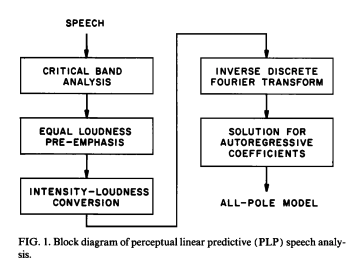
\includegraphics[width=0.50\textwidth]{figures/plp-analysis.png}
        \label{fig:/plp-block-diag}
    \end{figure}
    

    % Sub-problem 2
    \begin{subproblem}
        How do PLP coefficients differ from Mel frequency cepstral coefficients (MFCCs)?
    \end{subproblem}

    \textbf{Answer}

    Both PLP coeffients and MFCCs are commonly used feature representations for speech processing tasks such as speech recognition,
    speaker identification, and emotion detection. PLP and MFCCs are similar in thaht they both use a Mel filterbank to group spectral
    components of the speech signal into perceptually meaningful frequency bands. However, there are several key differences between
    the two feature representations.

    \begin{enumerate}
        \item Non-linear mapping: PLP coefficients use a  non-linear mapping of the filterbank outputs that is designed to better model the human auditoru system. in contracts, MFCCs use a linear transformation of the filterbank outputs.
        \item Cepstral smoothing: PLP coefficients use cepstral smoothing to reduce the effect of spectral noise and emphasise the format structure of the speech signal. In contrast MFCCs do not use cepstral smoothing.
        \item Spectral warping: PLP coefficients use a linear prediction model to estimate the spectral envelope of the speech signal, which can be used to further reduce the effects of spectral noise and improve the representation of the format structure. In contrast, MFCCs do not explicitly model the spectral envelope.
    \end{enumerate}

    In conclusion, PLP coefficients are designed to provide a more robust and accurate representation of the speech signal than MFCCs, 
    particularly in noisy or reverberant environments. However, the choice of feature representation ultimately depends on the specific
    application and the characteristics of the speech data being processed.

    \begin{mytheo}{What is a spectral envelope?}{theoexample}
        The spectral envelope of a speech signal refers to the shape of the overall spectral energy distribution across the frequency range of the speech signal. It represents the underlying pattern of resonances in the vocal tract, which are responsible for shaping the sounds of speech.
        
        The spectral envelope is called an "envelope" because it encloses the spectral shape of the speech signal, much like an envelope encloses a letter. It is a smooth function that describes the overall shape of the spectrum of the speech signal, without providing detailed information about individual spectral components.

        The spectral envelope can be estimated using various techniques, such as linear predictive coding (LPC), which models the speech signal as a linear combination of past samples, or the homomorphic filtering approach, which uses a logarithmic transformation of the speech signal to separate the spectral envelope from the fine spectral structure.

        Estimating the spectral envelope is important for many speech processing tasks, such as speech enhancement, speaker identification, and speech synthesis, because it provides a compact and informative representation of the underlying vocal tract characteristics that are responsible for the sound of speech. By modeling the spectral envelope, it is possible to separate the information that is most relevant to the perceptual quality of the speech signal from irrelevant or noisy spectral components.
    \end{mytheo}
    \FloatBarrier


    % Sub-problem 3
    \begin{subproblem}
        Which parts of the PLP computation are inspired by properties of human perception?
    \end{subproblem}

    \textbf{Answer}

    The PLP feature extraction method is designed to mimick the properties of human auditory perception, particularly with respect to the
    non-linearities and frequency selectivity of the auditory system. Several parts of the PLP computation are directly inspired by properties
    of human perception, including.

    \begin{enumerate}
        \item Mel filtering bank: the Mel filtering bank used in PLP is inspired by the frequency selectivity of the human cochlea, which acts as a bank of bandpass filters that seperate the incoming sound wave into narrow frequency bands. The mel scale is used to approximate the non-linear frequency spacing of the cochlea, which are more closely spaced at lower frequencies than at higher frequencies.
        \item Non-linear mapping: the non-linear mapping used in PLP is designed to mimic the compressive non-linearity of the inner hair cells in the cochlea, which act to increase the dynamic range of high level sounds.
        \item Cepstral smoothing: the cepstral smoothing used in PLP is designed to model the effect of the integration time constant of the auditory system, which causes rapid fluctuations in the spectral envelope to be smoothed out over time.
        \item Linear prediction: the linear prediction model used in PLP to estimate the spectral envelope is based on the idea that the vocal tract can be modeled as a linear fikter with time-varying coefficients, which can be estimated from the speech signal.
    \end{enumerate}

    By incorporating these perceptually inspired processing steps, PLP is able to provide a more accurate and robust representation of the human auditory system.

    \begin{mytheo}{What is a Mel frequency bank?}{theoexample}
        The Mel frequency bank is a collection of bandpass filters that are used to group the spectral components of a speech signal into perceptually meaningful frequency bands. The Mel frequency bank is based on the Mel scale, which is a non-linear scale of frequency that approximates the frequency spacing of the human auditory system.

        The Mel scale is designed to mimic the frequency selectivity of the human cochlea, which is the organ in the inner ear responsible for transducing sound into neural signals. The cochlea contains a bank of bandpass filters that separate the incoming sound wave into narrow frequency bands, with the bandwidth of each filter increasing with frequency.

        The Mel scale is based on the observation that the frequency spacing of these cochlear filters is non-uniform, with smaller frequency intervals at low frequencies and larger intervals at high frequencies. The Mel scale is defined such that the distance between two frequencies on the Mel scale corresponds to the difference in pitch that is perceived by the human ear.

        To construct the Mel frequency bank, a set of triangular bandpass filters are placed evenly spaced on the Mel scale, with the center frequencies of each filter corresponding to the peak of each triangle. The bandwidth of each filter is determined by the width of the triangle, which is typically chosen such that adjacent filters overlap slightly.

        The output of the Mel frequency bank is a set of filterbank coefficients, which represent the energy in each frequency band. These coefficients can be used as features in speech processing tasks such as speech recognition or speaker identification. The Mel frequency bank is a common pre-processing step for feature extraction methods such as Mel Frequency Cepstral Coefficients (MFCCs) or Perceptual Linear Prediction (PLP).
        
    \end{mytheo}


    % Sub-problem 4
    \begin{subproblem}
        Describe two ways in which information from multiple frames of the speech
        signal may be incorporated in the acoustic features used for an HMM /
        GMM (hidden Markov model / Gaussian mixture model) acoustic model,
        in order for the features to encode information about the speech dynamics
    \end{subproblem}

    \textbf{Answer}

    in order to capture the temporal dynamics of speech, it is often necessary to incorporate information from multiple frames of the speech
    signal into the acoustic features used fir an HMM/GMM acoustic model. Here are two ways in which this can be done.
    
    \begin{enumerate}
        \item Dynamic features: dunamic features are a class of acoustic features that incorporate information from multiple adjecent frames
        of the speech signal. One common type of dynamic feature is the delta feature, which represents the rate of change of the acoustic
        features over time. Delta features are computed by taking the first-order difference of the original acoustic features between
        adjacent frames. Another type of dynamic feature is the delta-delta feature, which represents the acceleration of the acoustic features 
        over time. Delta-delta features are computed by taking the second-order difference of the original acoustic features between adjecent
        frames. By incorporating information from multiple frames of the speech signal in this way, dynamic features can capture the temporal 
        dynamics of speech, such as changes in pitch, \textbf{formant transitions}, and coarticulation effects.

        \item Contextual features: are a class of acoustic features that incorporate information from neighboring frames of the speech signal, both 
        preceding  and following the current frame. Contextual features can be computed using a sliding window approach, where the acoustic features
        for each frame are concatenated with the features from neighboring with the features for neighboring frames within a certain window size. By
        incorporating contextual information from multiple frames of the speech signal in this way, contextual features can capture the contextual
        dependencies between adjecent speech sounds, such as phoneme-to-phoneme transitions or word-to-word transitions. One common type of contextual
        feature is the delta delayed feature, which incorporates information from both preceding and following frames of the speech signal to capture 
        the coarticulation effects between adjecent speech sounds.
    \end{enumerate}

    \begin{mytheo}{What are formant transitions?}{theoexample}
        Formant transitions are changes in the resonant frequencies of the vocal tract that occur during the production of speech sounds. Formants are the peaks in the frequency spectrum of a speech signal that correspond to the resonant frequencies of the vocal tract. The formants are determined by the shape and size of the vocal tract, which can be modified by the position and movement of the tongue, lips, and other articulators.

        When producing a speech sound, the vocal tract undergoes a series of rapid changes in shape as the articulators move to produce different phonemes. These changes cause the formant frequencies to shift, creating formant transitions between adjacent speech sounds. Formant transitions are particularly important for distinguishing between similar-sounding phonemes, such as /b/ and /p/, which differ primarily in the timing and direction of their formant transitions.

        Formant transitions can be captured in the acoustic features used for speech processing tasks such as speech recognition or speaker identification. Dynamic features such as delta and delta-delta features can be used to capture the rate of change of the formant frequencies over time, while contextual features such as pitch-synchronous features can be used to capture the pitch-dependent changes in the formant frequencies. Modeling formant transitions is an important aspect of acoustic modeling for speech processing, as it can help improve the accuracy and robustness of speech recognition and other speech processing tasks.
    \end{mytheo}

    \begin{mytheo}{What are coarticulation effects?}{theoexample}
        Coarticulation effects are changes in the acoustic properties of speech sounds that are caused by the influence of neighboring sounds in a sequence of speech. When we speak, we don't produce each sound in isolation; instead, the production of one sound can influence the production of the sounds that come before and after it. Coarticulation effects can include changes in the timing, duration, amplitude, and spectral characteristics of speech sounds.

        For example, when producing the word "bat," the articulation of the consonant /b/ requires the lips to be pressed together, which affects the shape and size of the vocal tract. As a result, the formant frequencies of the following vowel /a/ are shifted slightly compared to the formants of the same vowel produced in isolation. Similarly, when producing the word "cab," the articulation of the consonant /k/ requires the tongue to be pressed against the velum, which affects the shape and size of the vocal tract and causes a shift in the formant frequencies of the preceding vowel /æ/.

        Coarticulation effects can make speech recognition and other speech processing tasks more challenging, as the acoustic properties of a given speech sound can vary depending on the sounds that come before and after it. However, coarticulation effects can also provide useful information for understanding the dynamics of speech production and for developing more accurate and robust models of speech processing. Dynamic and contextual features, as well as other acoustic modeling techniques, can be used to capture coarticulation effects and improve the accuracy of speech processing algorithms.
    \end{mytheo}


    % Sub-problem 5 
    \begin{subproblem}
        In hybrid HMM / DNN (hidden Markov model / deep neural network)
        systems, log mel filterbank features have been found to be superior to PLP
        coefficients or MFCCs (mel frequency cepstral coefficients). Why might this
        be the case, and why is it not the case for HMM / GMM systems?
    \end{subproblem}

    \textbf{Answer}

    Log mel filterbank features have been found to be superior to PLP coefficients or MFCCs in hybrid HMM/DNN systems for several reasons.

    \begin{enumerate}
        \item Better representation of spectral information: log mel filterbanks better represent the spectral information in speech signals compared to other features like MFCCs or PLPs.
        this is because the human auditory system is more sensitive to changes in frequency at lower frequencies than at higher frequencies, and log mel filterbanks capture this property
        by mapping the spectral frequenices into mel-scale, whoch is logarithmically spaced at lower frequencies and linearly spread at higher frequencies.

        \item More robust to noise: log mel filterbanks are more robust to additive noise then MFCCs and PLPs This is because they are less sensitve to changes in the amplitude of the
        signal and more sensitive to changes in the spectral shape.
        
        \item Better regularisation: the use of log mel filterbanks as input to DNNs provides better regularisation than PLPs or MFCCs. This is because the number of parameters in a DNN
        is much larger then in an HMM, and the use of log mel filterbanks helps to reduce overfitting by providing a more compact representation of the spectral information.
    \end{enumerate}

    However, the superiority of log mel filterbanks over other features is not always the case for HMM/GMM systems. This is because HMM/GMM systems are based in Gaussian mixture models (GMMs)
    that assume the statistical distribution of the features in Gaussian. In this case, the use of PLPs or MFCCs may provide a better fir to the Gaussian distribution assumption of the GMM.
    In addition, HMM/GMM systems are typically trained using maximum likelihood estimation (MLE), which is less sensitive to the choice of input features than DNN-based systems.

\end{homeworkProblem}


% Problem 2
\begin{homeworkProblem}
    
    % Sub-problem 1
    \begin{subproblem}
        Consider a hidden Markov model (HMM) which has a state output distribution given by a single Gaussian. We would like to estimate the mean
        $\mu_j$ of state $s_j$, given a training sequence of acoustic observations $X =x_1, \ldots, x_t, \ldots, x_T$.

        If the time-state alignment is known, write an expression for the maximum likelihood estimate of $\mu_j$.
    \end{subproblem}

    \textbf{Answer}

    The expression for the estimated $\mu_j$, given that we have a single Gaussian optimised using MLE is given by.

    \begin{align}
        \mu_j = \displaystyle\frac{1}{T} \displaystyle\sum_{T}^{t=1} x_t
    \end{align}

\end{homeworkProblem}

\end{document}
